\chapter{Pod}


A pod is a group of one or more tightly related containers that will always run together on the same worker node and in the same Linux namespace(s). Each pod is like a separate logical machine with its own IP, hostname, processes, and so on, running a single \emph{application}. The application can be a single process, running in a single container, or it can be a main application process and additional supporting processes, each running in its own container. All the containers in a pod will apear to be running on the same logical machine, whereas containers in other pods, even if they're running on the same worker node, will appear to be running on a different one.

A special service of type LoadBalancer.


The host name of the application is the name of the pod as each pod behaves like a separate independent machine with its own IP address and hostname.

\begin{remark}
	As we can see here that the underlying low-level architecture is completely hidden from developers.
\end{remark}

\begin{itemize}
	\item The basic building block in Kubernetes is the pod.
	\item To make that pod accessbiel from outside the cluster, you need to tell Kubernetes to expose all the pods managed by that ReplicationController as a single Service.
	\item The pod has its own unique private IP address and hostname.
	\item A key characteristic of pods is that tey are ephemeral. A pod may disappear at any time \textemdash because the node it's running on has failed, because someone deleted the pod, or because the pod was evicted from an otherwise healthey node. When any of those occurs, a missing pod is replaced with a new one by the ReplicationController. This new pod gets a different IP address from the pod it's replacing. This is where services com in \textemdash to solve the problem of ever-changing pod IP addresses, as well as exposing multiple pods at a single constant IP and port pair.
\end{itemize}



\begin{center}
	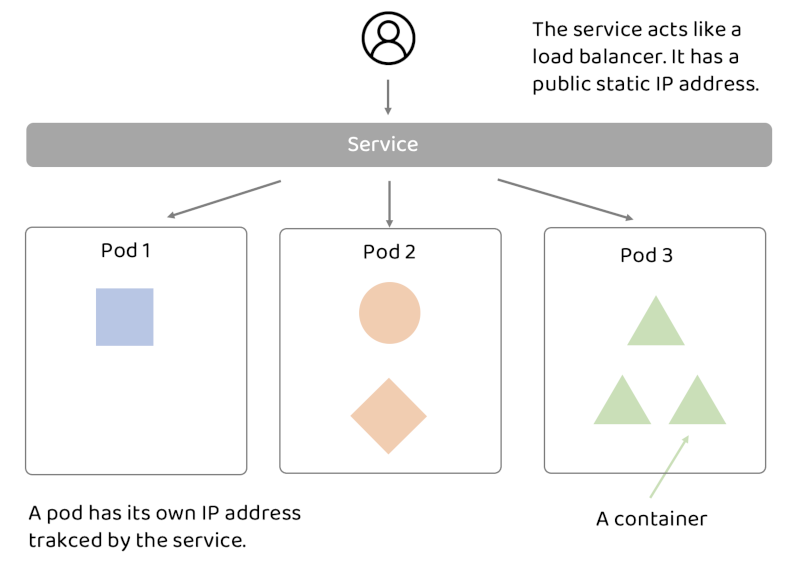
\includegraphics[max width=\textwidth]{pod/k8s_service_and_pod.png}
\end{center}
